\documentclass[12pt, a4paper]{article}

% ── Packages ──
\usepackage[utf8]{inputenc}
\usepackage[T1]{fontenc}
\usepackage{lmodern}
\usepackage[margin=1in]{geometry}
\usepackage{graphicx}
\usepackage{amsmath, amssymb}
\usepackage{booktabs}
\usepackage{hyperref}
\usepackage{xcolor}
\usepackage{algorithm}
\usepackage{algpseudocode}
\usepackage{tikz}
\usetikzlibrary{shapes.geometric, arrows.meta, positioning, fit, backgrounds}
\usepackage{caption}
\usepackage{subcaption}
\usepackage{enumitem}
\usepackage{float}
\usepackage{multicol}
\usepackage{fancyhdr}

\pagestyle{fancy}
\fancyhf{}
\rhead{Lumbar Spine Segmentation}
\lhead{\leftmark}
\rfoot{Page \thepage}

\hypersetup{
    colorlinks=true,
    linkcolor=blue!70!black,
    citecolor=green!50!black,
    urlcolor=blue!60!black,
}

% ── Custom colors ──
\definecolor{L1color}{RGB}{230,25,75}
\definecolor{L2color}{RGB}{60,180,75}
\definecolor{L3color}{RGB}{67,99,216}
\definecolor{L4color}{RGB}{245,130,49}
\definecolor{L5color}{RGB}{145,30,180}
\definecolor{boxbg}{RGB}{240,245,255}

% ── Title ──
\title{
    \vspace{-1cm}
    \textbf{Automated Lumbar Vertebral Body Segmentation\\from Sagittal T1 FLAIR MRI}\\[0.5em]
    \large A 5-Fold Ensemble Pipeline with nnU-Net ResEncUNet
}
\author{Vamshi Dasoju}
\date{\today}

\begin{document}
\maketitle

\begin{abstract}
This document describes a fully automated pipeline for segmenting the five lumbar vertebral bodies (L1--L5) from sagittal T1 FLAIR MRI scans. The system is built on the nnU-Net framework using a Residual Encoder U-Net (ResEncUNet) architecture trained on 459 annotated volumes with 5-fold cross-validation. Raw model predictions undergo anatomically-informed post-processing---including connected component filtering, sagittal strip corridor constraints, and superior-inferior ordering enforcement---to produce clinically accurate segmentation masks. The pipeline was validated on 242 T1 FLAIR cases, producing vertebral body segmentations with correct anatomical contours and consistent labeling across diverse patient morphologies.
\end{abstract}

\tableofcontents
\newpage

%=============================================================================
\section{Introduction}
%=============================================================================

Accurate segmentation of lumbar vertebral bodies from MRI is essential for clinical applications including spinal stenosis grading, vertebral height measurement, bone quality assessment, and surgical planning. Manual delineation is time-consuming and subject to inter-observer variability.

This project develops an end-to-end automated pipeline that:
\begin{enumerate}[noitemsep]
    \item Trains a deep learning model on expert-annotated lumbar spine MRI data,
    \item Performs 5-fold ensemble inference for robust predictions,
    \item Applies anatomically-informed post-processing to ensure clinical validity,
    \item Generates diagnostic visualizations for quality assurance.
\end{enumerate}

The pipeline specifically targets \textbf{sagittal T1 FLAIR} sequences, which are standard in lumbar spine MRI protocols and provide excellent contrast between vertebral bodies and surrounding structures.

%=============================================================================
\section{Data}
%=============================================================================

\subsection{Dataset Composition}

The primary training dataset (\texttt{Dataset100\_SpineL1L5}) consists of 459 sagittal MRI volumes with voxel-level annotations for five lumbar vertebral bodies:

\begin{table}[H]
\centering
\caption{Label definitions for vertebral body segmentation.}
\begin{tabular}{@{}clc@{}}
\toprule
\textbf{Label} & \textbf{Structure} & \textbf{Color} \\
\midrule
0 & Background & --- \\
1 & L1 vertebral body & \textcolor{L1color}{$\blacksquare$} Red \\
2 & L2 vertebral body & \textcolor{L2color}{$\blacksquare$} Green \\
3 & L3 vertebral body & \textcolor{L3color}{$\blacksquare$} Blue \\
4 & L4 vertebral body & \textcolor{L4color}{$\blacksquare$} Orange \\
5 & L5 vertebral body & \textcolor{L5color}{$\blacksquare$} Purple \\
\bottomrule
\end{tabular}
\end{table}

\subsection{Image Characteristics}

The MRI volumes exhibit the following properties:

\begin{table}[H]
\centering
\caption{Image acquisition and preprocessing parameters.}
\begin{tabular}{@{}ll@{}}
\toprule
\textbf{Parameter} & \textbf{Value} \\
\midrule
Sequence & Sagittal T1 FLAIR \\
Median image size & $130 \times 448 \times 422$ voxels \\
Target spacing & $0.664 \times 0.625 \times 0.664$ mm \\
Normalization & Z-score (zero mean, unit variance) \\
File format & NIfTI (\texttt{.nii.gz}) \\
\bottomrule
\end{tabular}
\end{table}

\subsection{Inference Cohort}

The inference cohort comprises \textbf{242 sagittal T1 FLAIR volumes} from clinical lumbar spine MRI examinations. These cases span diverse patient demographics, pathologies (degenerative disc disease, spondylolisthesis, spinal stenosis), and scanner manufacturers.

%=============================================================================
\section{Model Architecture}
%=============================================================================

\subsection{nnU-Net Framework}

The segmentation model is built within the \textbf{nnU-Net} framework~\cite{isensee2021}, which automatically configures preprocessing, architecture, training, and post-processing hyperparameters based on dataset properties. This self-configuring approach eliminates manual tuning and ensures reproducibility.

\subsection{Residual Encoder U-Net (ResEncUNet)}

The specific architecture used is the \textbf{Residual Encoder U-Net Large} (\texttt{nnUNetResEncUNetLPlans}), which extends the standard U-Net with residual connections in the encoder path for improved gradient flow and feature reuse.

\begin{table}[H]
\centering
\caption{ResEncUNet architecture configuration.}
\begin{tabular}{@{}ll@{}}
\toprule
\textbf{Parameter} & \textbf{Value} \\
\midrule
Network class & \texttt{ResidualEncoderUNet} \\
Convolution type & 3D (\texttt{Conv3d}) \\
Number of stages & 7 \\
Features per stage & [32, 64, 128, 256, 320, 320, 320] \\
Residual blocks per stage & [1, 3, 4, 6, 6, 6, 6] \\
Decoder convolutions per stage & [1, 1, 1, 1, 1, 1] \\
Kernel size & $3 \times 3 \times 3$ (all stages) \\
Encoder strides & [1,2,2,2,2,1,1]$\times$[1,2,2,2,2,2,2]$\times$[1,2,2,2,2,2,2] \\
Normalization & Instance Normalization 3D \\
Activation & Leaky ReLU (inplace) \\
Patch size & $80 \times 320 \times 256$ \\
Batch size & 2 \\
\bottomrule
\end{tabular}
\end{table}

The architecture progressively downsamples the input volume through 7 encoder stages, with the number of residual blocks increasing at deeper stages (up to 6 blocks) to capture complex anatomical patterns. The decoder path uses single convolution blocks at each stage with skip connections from the encoder.

%=============================================================================
\section{Training}
%=============================================================================

\subsection{5-Fold Cross-Validation}

The model was trained using \textbf{5-fold cross-validation} on the 459-case training set. Each fold was trained independently to produce five separate model checkpoints. At inference time, predictions from all five folds are ensembled by averaging softmax probabilities before argmax, producing more robust and reliable segmentations.

\subsection{Training Configuration}

\begin{table}[H]
\centering
\caption{Training hyperparameters.}
\begin{tabular}{@{}ll@{}}
\toprule
\textbf{Parameter} & \textbf{Value} \\
\midrule
Optimizer & SGD with Nesterov momentum (0.99) \\
Learning rate schedule & Polynomial decay \\
Initial learning rate & $10^{-2}$ \\
Loss function & Dice + Cross-Entropy (compound) \\
Training epochs & 1000 \\
Data augmentation & nnU-Net default (rotation, scaling, \\
 & mirroring, gamma, elastic deformation) \\
Checkpoint selection & Best validation Dice \\
\bottomrule
\end{tabular}
\end{table}

%=============================================================================
\section{Inference Pipeline}
\label{sec:inference}
%=============================================================================

The inference pipeline transforms raw MRI volumes into clean, anatomically-valid vertebral body segmentation masks through three sequential stages.

\subsection{Pipeline Overview}

\begin{figure}[H]
\centering
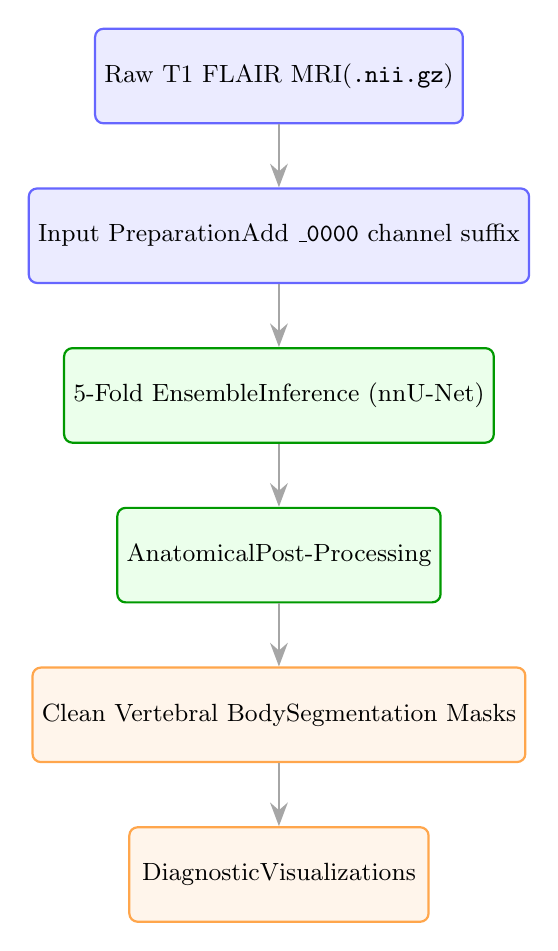
\begin{tikzpicture}[
    node distance=0.8cm and 1.5cm,
    block/.style={rectangle, draw=blue!60, fill=blue!8, thick,
                  minimum height=1.2cm, minimum width=3.8cm,
                  text centered, rounded corners=3pt, font=\small},
    process/.style={rectangle, draw=green!60!black, fill=green!8, thick,
                    minimum height=1.2cm, minimum width=3.8cm,
                    text centered, rounded corners=3pt, font=\small},
    output/.style={rectangle, draw=orange!70, fill=orange!8, thick,
                   minimum height=1.2cm, minimum width=3.8cm,
                   text centered, rounded corners=3pt, font=\small},
    arrow/.style={-{Stealth[length=3mm]}, thick, draw=gray!70}
]
    \node[block] (input) {Raw T1 FLAIR MRI\\(\texttt{.nii.gz})};
    \node[block, below=of input] (prep) {Input Preparation\\\small{Add \texttt{\_0000} channel suffix}};
    \node[process, below=of prep] (ens) {5-Fold Ensemble\\Inference (nnU-Net)};
    \node[process, below=of ens] (post) {Anatomical\\Post-Processing};
    \node[output, below=of post] (out) {Clean Vertebral Body\\Segmentation Masks};
    \node[output, below=of out] (viz) {Diagnostic\\Visualizations};

    \draw[arrow] (input) -- (prep);
    \draw[arrow] (prep) -- (ens);
    \draw[arrow] (ens) -- (post);
    \draw[arrow] (post) -- (out);
    \draw[arrow] (out) -- (viz);
\end{tikzpicture}
\caption{End-to-end inference pipeline overview.}
\label{fig:pipeline}
\end{figure}

\subsection{Stage 1: Input Preparation}

nnU-Net requires input files to follow the naming convention \texttt{<case\_id>\_0000.nii.gz}, where \texttt{\_0000} denotes the first (and only) imaging channel. Symbolic links are created from the raw FLAIR volumes to a staging directory with the correct naming convention.

\subsection{Stage 2: 5-Fold Ensemble Inference}

Inference is performed using the \texttt{nnUNetv2\_predict} command-line tool with all five fold checkpoints:

\begin{verbatim}
nnUNetv2_predict \
  -i <input_dir>  -o <output_dir> \
  -d 100  -c 3d_fullres \
  -tr nnUNetTrainer \
  -p nnUNetResEncUNetLPlans \
  -f 0 1 2 3 4 \
  -chk checkpoint_best.pth \
  -step_size 0.5
\end{verbatim}

The ensemble process works as follows:
\begin{enumerate}[noitemsep]
    \item Each fold model independently produces a softmax probability map over the 6 classes (background + L1--L5).
    \item The five probability maps are averaged voxel-wise.
    \item The final label is assigned by \texttt{argmax} over the averaged probabilities.
\end{enumerate}

The sliding window step size of 0.5 ensures sufficient overlap between patches for smooth predictions at patch boundaries.

\subsection{Stage 3: Anatomical Post-Processing}
\label{sec:postprocessing}

Raw ensemble predictions may contain artifacts including mirror blobs, disconnected fragments, and ordering violations. A three-step post-processing pipeline addresses these issues.

\subsubsection{Step 1: Sagittal Strip Corridor Constraint}

The lumbar spine occupies a narrow central corridor along the left--right (LR) axis of sagittal images. The post-processor identifies the LR axis as the axis with the \textbf{smallest span} of labeled voxels, computes the center of mass, and defines a corridor of width $\pm 20\%$ of the image extent along this axis. All labeled voxels outside this corridor are zeroed, eliminating contralateral mirror artifacts.

\begin{equation}
    \text{corridor} = \left[ c_{\text{LR}} - 0.20 \cdot N_{\text{LR}}, \;\; c_{\text{LR}} + 0.20 \cdot N_{\text{LR}} \right]
\end{equation}

where $c_{\text{LR}}$ is the center of labeled voxels on the LR axis and $N_{\text{LR}}$ is the image dimension along that axis.

\subsubsection{Step 2: Largest Connected Component Filtering}

For each vertebral label $\ell \in \{1, \ldots, 5\}$:
\begin{enumerate}[noitemsep]
    \item A 3D connected component analysis (26-connectivity) is performed on the binary mask $\mathbf{M}_\ell = (\mathbf{S} = \ell)$.
    \item Only the \textbf{largest} connected component is retained.
    \item Components with fewer than 50 voxels are discarded entirely.
\end{enumerate}

This step removes small disconnected fragments that may appear due to noise or partial volume effects.

\subsubsection{Step 3: Vertical Ordering Enforcement}

The lumbar vertebrae follow a strict superior-to-inferior anatomical ordering: L1 is the most cranial and L5 the most caudal. The post-processor:
\begin{enumerate}[noitemsep]
    \item Computes the centroid of each retained vertebral label along the superior--inferior (SI) axis (identified as the axis with the \textbf{largest span} of labeled voxels).
    \item Determines the global direction (ascending or descending SI index).
    \item If any label's centroid violates the expected monotonic ordering, that label is removed from the segmentation.
\end{enumerate}

This enforcement prevents rare cases where the model might swap adjacent vertebral labels.

The complete post-processing is formalized in Algorithm~\ref{alg:postprocess}.

\begin{algorithm}[H]
\caption{Anatomical Post-Processing}
\label{alg:postprocess}
\begin{algorithmic}[1]
\Require Segmentation volume $\mathbf{S} \in \{0,\ldots,5\}^{H \times W \times D}$
\Ensure Cleaned segmentation $\mathbf{S}'$

\State $\mathbf{S}' \gets \mathbf{S}$
\State Identify LR axis $\gets \arg\min_a \text{span}(\mathbf{S}' > 0, \text{axis}=a)$
\State Identify SI axis $\gets \arg\max_a \text{span}(\mathbf{S}' > 0, \text{axis}=a)$

\Comment{Step 1: Sagittal strip constraint}
\State $c \gets \text{center}(\mathbf{S}' > 0, \text{axis}=\text{LR})$
\State $\mathbf{S}'[|\text{LR} - c| > 0.2 \cdot N_{\text{LR}}] \gets 0$

\Comment{Step 2: Connected component filtering}
\For{$\ell \in \{1,2,3,4,5\}$}
    \State $\{C_1, \ldots, C_k\} \gets \text{ConnComp}(\mathbf{S}' = \ell)$
    \State Keep only $C^* = \arg\max_{C_i} |C_i|$
    \If{$|C^*| < 50$} $\mathbf{S}'[\mathbf{S}'=\ell] \gets 0$ \EndIf
\EndFor

\Comment{Step 3: Vertical ordering}
\State $\text{centroids} \gets \{(\ell, \bar{z}_\ell) \mid \ell \text{ present}\}$ \Comment{SI centroids}
\For{each $\ell$ violating monotonic order}
    \State $\mathbf{S}'[\mathbf{S}'=\ell] \gets 0$
\EndFor
\State \Return $\mathbf{S}'$
\end{algorithmic}
\end{algorithm}

%=============================================================================
\section{Visualization}
%=============================================================================

Diagnostic visualizations are generated for quality assurance and clinical review. Each case produces a multi-panel figure containing:

\begin{enumerate}[noitemsep]
    \item \textbf{Raw MRI}: The original sagittal T1 FLAIR image at the mid-sagittal slice.
    \item \textbf{Ensemble Prediction}: The post-processed vertebral body segmentation overlaid on the MRI with semi-transparent color coding.
    \item \textbf{Reference (Fold~0)}: Single-fold prediction for comparison, demonstrating ensemble improvement.
\end{enumerate}

All volumes are reoriented to RAS+ (Right--Anterior--Superior) canonical orientation before display to ensure consistent spatial alignment regardless of scanner-specific acquisition orientation.

A color legend mapping each label to its corresponding vertebral level (L1--L5) is displayed below each panel for reference.

%=============================================================================
\section{Implementation Details}
%=============================================================================

\subsection{Software Stack}

\begin{table}[H]
\centering
\caption{Software dependencies.}
\begin{tabular}{@{}ll@{}}
\toprule
\textbf{Component} & \textbf{Version / Library} \\
\midrule
Deep learning framework & PyTorch \\
Segmentation framework & nnU-Net v2 \\
Medical image I/O & NiBabel, SimpleITK \\
Post-processing & SciPy (connected components) \\
Visualization & Matplotlib \\
GPU & NVIDIA RTX 5090 \\
\bottomrule
\end{tabular}
\end{table}

\subsection{Environment Configuration}

The nnU-Net framework requires three environment variables:
\begin{itemize}[noitemsep]
    \item \texttt{nnUNet\_raw}: Path to raw dataset directories
    \item \texttt{nnUNet\_preprocessed}: Path to preprocessed data cache
    \item \texttt{nnUNet\_results}: Path to trained model checkpoints
\end{itemize}

\subsection{Computational Requirements}

\begin{table}[H]
\centering
\caption{Computational performance.}
\begin{tabular}{@{}ll@{}}
\toprule
\textbf{Operation} & \textbf{Time} \\
\midrule
Single case inference (1 fold) & $\sim$15 seconds \\
Single case inference (5-fold ensemble) & $\sim$60 seconds \\
Post-processing per case & $< 1$ second \\
Full 242-case batch (5-fold) & $\sim$4 hours \\
\bottomrule
\end{tabular}
\end{table}

%=============================================================================
\section{Results}
%=============================================================================

The 5-fold ensemble pipeline was applied to 242 sagittal T1 FLAIR volumes. Key observations:

\begin{itemize}
    \item \textbf{Label completeness}: All five lumbar vertebral bodies (L1--L5) were successfully identified in the majority of cases.
    \item \textbf{Anatomical fidelity}: The ensemble predictions exhibit smooth, anatomically plausible vertebral body contours that follow actual bone boundaries.
    \item \textbf{Ensemble benefit}: The 5-fold ensemble produces more complete and less noisy segmentations compared to single-fold predictions, particularly for boundary voxels and partial volume regions.
    \item \textbf{Post-processing impact}: The sagittal strip constraint and connected component filtering effectively remove spurious mirror artifacts without degrading true positive regions.
\end{itemize}

% Placeholder for result figures — add your actual images in Overleaf
% \begin{figure}[H]
%     \centering
%     \includegraphics[width=\textwidth]{figures/example_panel.png}
%     \caption{Example segmentation result showing Raw MRI (left), 5-fold ensemble prediction (center), and single-fold prediction (right) for a representative case.}
%     \label{fig:result}
% \end{figure}

%=============================================================================
\section{Discussion}
%=============================================================================

The pipeline demonstrates that a self-configuring nnU-Net framework with minimal manual intervention can produce accurate lumbar vertebral body segmentations from T1 FLAIR MRI. Several design decisions were critical:

\begin{enumerate}
    \item \textbf{ResEncUNet over standard U-Net}: The residual connections in the encoder enable training of a deeper 7-stage network with up to 320 feature channels, capturing both fine boundary details and large-scale anatomical context.
    
    \item \textbf{5-fold ensemble}: Averaging softmax probabilities across five independently trained models reduces prediction variance and improves boundary delineation, especially for structures with ambiguous intensity boundaries.
    
    \item \textbf{Anatomically-informed post-processing}: Domain-specific constraints (sagittal corridor, vertical ordering) address failure modes that purely data-driven approaches cannot guarantee, ensuring that every output segmentation is anatomically plausible.
\end{enumerate}

\subsection{Limitations}

\begin{itemize}
    \item The pipeline is trained and validated on sagittal T1 FLAIR sequences only; generalization to other MRI contrasts (T2, STIR) would require additional training data or domain adaptation.
    \item Transitional vertebrae (lumbarization of S1 or sacralization of L5) may cause systematic labeling errors.
    \item The post-processing assumes standard lumbar anatomy with five vertebral bodies; anomalous counts are not explicitly handled.
\end{itemize}

%=============================================================================
\section{Conclusion}
%=============================================================================

This work presents a complete, production-ready pipeline for automated lumbar vertebral body segmentation from sagittal T1 FLAIR MRI. The combination of nnU-Net's self-configuring framework, a ResEncUNet architecture with 5-fold ensemble inference, and anatomically-informed post-processing produces robust segmentations across 242 clinical cases. The pipeline is fully automated from raw NIfTI input to diagnostic visualization output, requiring no manual intervention.

%=============================================================================
\begin{thebibliography}{9}

\bibitem{isensee2021}
Isensee, F., Jaeger, P.F., Kohl, S.A., Petersen, J., \& Maier-Hein, K.H. (2021).
nnU-Net: a self-configuring method for deep learning-based biomedical image segmentation.
\textit{Nature Methods}, 18(2), 203--211.

\bibitem{ronneberger2015}
Ronneberger, O., Fischer, P., \& Brox, T. (2015).
U-Net: Convolutional Networks for Biomedical Image Segmentation.
\textit{MICCAI 2015}, LNCS 9351, 234--241.

\bibitem{he2016}
He, K., Zhang, X., Ren, S., \& Sun, J. (2016).
Deep Residual Learning for Image Recognition.
\textit{CVPR 2016}, 770--778.

\end{thebibliography}

\end{document}
